\documentclass[11pt]{article}
\usepackage[hmargin={1in},vmargin={1in,1in}]{geometry}   
\geometry{letterpaper}            
\usepackage[parfill]{parskip}
\usepackage{color,graphicx}
\usepackage{setspace}
\usepackage{amsmath}
\usepackage{amssymb}
\usepackage{textcomp}
\usepackage{linguex}
\usepackage{multirow}
\usepackage{pifont}
\usepackage{natbib}
\usepackage[normalem]{ulem}
\usepackage{wrapfig}

\usepackage{fancyhdr}
\lhead{Scontras, Degen \& Goodman}\chead{}\rhead{Adjective ordering}
\renewcommand{\headrulewidth}{.3pt}
\lfoot{}\cfoot{\thepage}\rfoot{}
\newcommand{\txtp}{\textipa}
\renewcommand{\rm}{\textrm}
\newcommand{\sem}[1]{\mbox{$[\![$#1$]\!]$}}
\newcommand{\lam}{$\lambda$}
\newcommand{\lan}{$\langle$}
\newcommand{\ran}{$\rangle$}
\newcommand{\type}[1]{\ensuremath{\left \langle #1 \right \rangle }}
\newcommand{\defeq}{$\mathrel{\mathop:}=$ }
\renewcommand{\and}{$\wedge$ }

\newcommand{\bex}{\begin{examples}}
\newcommand{\eex}{\end{examples}}
\newcommand{\bit}{\begin{itemize}}
\newcommand{\eit}{\end{itemize}}
\newcommand{\ben}{\begin{enumerate}}
\newcommand{\een}{\end{enumerate}}

\renewcommand{\bibsection}{}

\pagestyle{fancy}

\title{Adjective Ordering}
\author{Gregory Scontras, Judith Degen, and Noah D.~Goodman}
\date{\today}


\begin{document}

\thispagestyle{plain}

\maketitle

\begin{abstract}
	Here is the abstract
\end{abstract}


\section{Introduction}

Background on adjective ordering preferences

\subsection{English}

\subsection{Cross-linguistic stability}


\section{Corpus work} \label{corpus}


\section{Experiments}

\subsection{Ordering preferences}

\subsubsection{Participants}

We recruited 50 participants through Amazon.com's Mechanical Turk crowd-sourcing service. Participants were compensated for their participation.

\subsubsection{Design and methods}

Participants were asked to decide which of two descriptions of an object sounded more natural. Each description featured a noun modified by two adjectives, for example ``the red small chair'' or ``the small red chair''. Description pairs contained the same words, with relative adjective order reversed. Descriptions were random combinations of two adjectives and a noun from the list in Table \ref{stim-table} (compiled via the procedure described in Section \ref{corpus} above), with the constraint that no description contained adjectives from the same adjective class.

\begin{table}
	\centering
	\caption{Adjectives and nouns used in experimental stimuli.}\label{stim-table}
	\begin{tabular}{llc||cll}\hline
		\textsc{adjective} & \textsc{class} &&& \textsc{noun} & \textsc{class}\\\hline
				red & color &&& apple & food \\
				yellow & color &&& banana & food \\
				green & color &&& carrot & food \\
				blue & color &&& cheese & food \\
				purple & color &&& tomato & food \\
				brown & color &&& chair & furniture \\					
				big & size &&& couch & furniture \\
				small & size &&& fan & furniture \\					
				huge & size &&& TV & furniture \\					
				tiny & size &&& desk & furniture \\					
				short & size &&& \\					
				long & size &&& 	\\						
				wooden & material &&& \\
				plastic & material &&& \\
				metal & material &&& \\
				smooth & texture &&& \\
				hard & texture &&& \\
				soft & texture &&& \\
				old & age &&& \\
				new & age &&& \\
				rotten & age &&&\\ 
				fresh & age &&& \\
				good & quality &&& \\
				bad & quality &&& \\
				round & shape &&&\\ 						
				square & shape &&&\\ 
		\end{tabular}
\end{table}

On each trial, participants indicated which description sounded more natural by adjusting a slider whose endpoints were labeled with the competing descriptions (Fig.~\ref{order-trial})

\begin{figure}[h!]
\centering
	\fbox{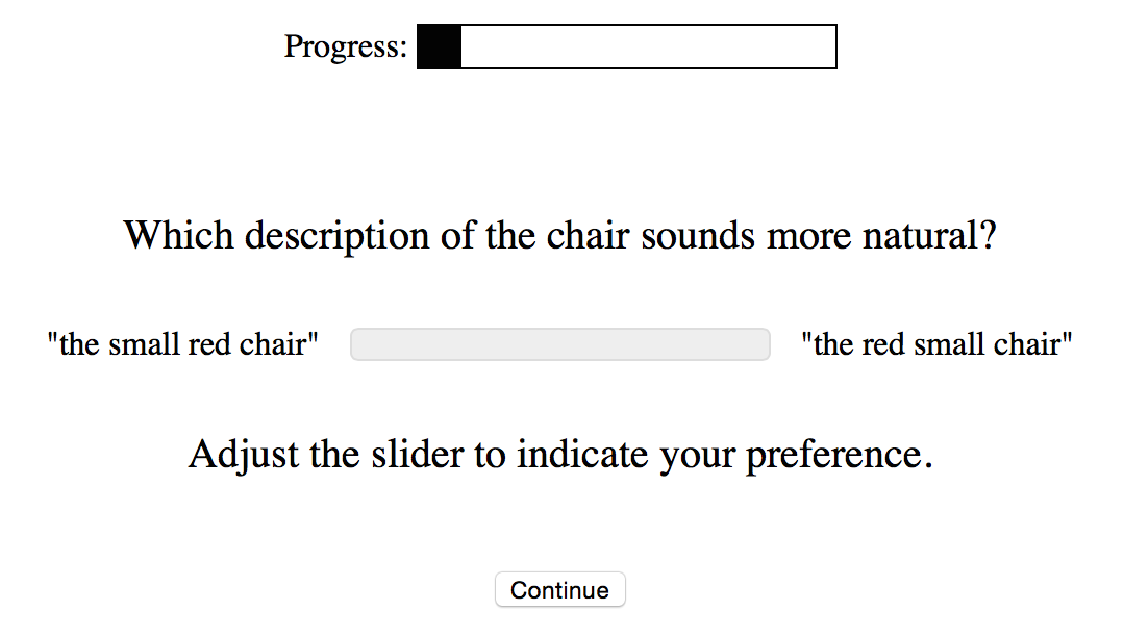
\includegraphics[width=.8\linewidth]{images/order_trial.eps}}
	\caption{Example trial from Expt.~1; participants chose the more natural of two adjective-adjective-noun descriptions, which differed in the relative ordering of the two adjectives.}\label{order-trial}
\end{figure}

\subsubsection{Predictions}

\subsubsection{Results}

\subsubsection{Discussion}


\subsection{Faultless disagreement}

\subsubsection{Participants}

\subsubsection{Design and methods}

\subsubsection{Predictions}

\subsubsection{Results}

\subsubsection{Discussion}


\subsection{Predicting ordering preferences with faultless disagreement}



\section{Possible accounts}


\subsection{Memory}

Forgetting account

\subsection{Syntax}

John Beavers spray/load work

\subsection{UID}

Different notions of informativity

\subsection{Flexibility}

\emph{Blue} is less subjective so I rarely speak of ``blue for X'', whereas more subjective and flexible \emph{good} is often spoken of in terms of ``good for Y''.


\section{General discussion}


\end{document}